% =====================================================================
%  M.Tech / Master's Thesis Report Template
%  Modelled on the IIT Guwahati (CSE) M.Tech project report format.
%  Compile:  pdflatex main && bibtex main && pdflatex main && pdflatex main
%  (or simply:  latexmk -pdf main)
% =====================================================================
\documentclass[12pt,a4paper,oneside]{report}

% ---------------------------------------------------------------------
%  1.  THESIS DETAILS  -- edit these fields only
% ---------------------------------------------------------------------
\newcommand{\thesistitle}{Security Analysis of\\ Lower-Layer Triggered Mobility\\ in 5G-Advanced and 6G Networks}
\newcommand{\thesistitleflat}{Security Analysis of Lower-Layer Triggered Mobility in 5G-Advanced and 6G Networks} % single-line, for the certificate
\newcommand{\degreename}{Master of Technology}
\newcommand{\reporttype}{M.\ Tech Project Report (Phase I)}   % e.g. M.\ Tech Thesis, MS Thesis
\newcommand{\authorname}{Pranjal Chouhan}
\newcommand{\rollno}{254101040}
\newcommand{\supervisorname}{Prof.\ Moumita Patra}
\newcommand{\supervisortitle}{Department of Computer Science \& Engineering}
\newcommand{\departmentname}{Department of Computer Science \& Engineering}
\newcommand{\departmentcaps}{DEPARTMENT OF COMPUTER SCIENCE AND ENGINEERING}
\newcommand{\institutecaps}{INDIAN INSTITUTE OF TECHNOLOGY GUWAHATI}
\newcommand{\institutename}{Indian Institute of Technology Guwahati}
\newcommand{\institutecity}{GUWAHATI - 781039, ASSAM}
\newcommand{\submissiondate}{November, 2026}
\newcommand{\submissionplace}{Guwahati}
\newcommand{\logofile}{figures/iitg_logo.png}        % put your institute logo here

% ---------------------------------------------------------------------
%  2.  PACKAGES
% ---------------------------------------------------------------------
\usepackage[T1]{fontenc}
\usepackage[utf8]{inputenc}
\usepackage{lmodern}
\usepackage[a4paper,left=3.0cm,right=2.5cm,top=2.5cm,bottom=2.5cm]{geometry}
\usepackage{setspace}
\usepackage{microtype}

% math
\usepackage{amsmath,amssymb,amsfonts,mathtools}

% graphics, tables, floats
\usepackage{graphicx}
\usepackage{booktabs}
\usepackage{tabularx}
\usepackage{longtable}
\usepackage{etoolbox}
\usepackage{multirow}
\usepackage{array}
\usepackage{xcolor}
\usepackage{float}
\usepackage[font=small,labelfont=bf,labelsep=colon]{caption}
\captionsetup[figure]{name=Fig.}
\captionsetup[table]{position=above}
\usepackage{subcaption}

% code listings
\usepackage{listings}
\lstset{basicstyle=\ttfamily\small,breaklines=true,frame=single,
        numbers=left,numberstyle=\tiny,keywordstyle=\color{blue!70!black},
        commentstyle=\color{green!40!black},showstringspaces=false}

% headings and page style
\usepackage{titlesec}
\usepackage{fancyhdr}

% bibliography: numeric, IEEE style ([1], [2, 3])
\usepackage[nocompress]{cite}
% tighter bibliography list
\apptocmd{\thebibliography}{\setlength{\itemsep}{0pt plus 0.2pt}\setlength{\parsep}{0pt}}{}{}

% links (load late)
\usepackage[hidelinks]{hyperref}
\usepackage[nameinlink,capitalise,noabbrev]{cleveref}
\crefname{figure}{Figure}{Figures}

% ---------------------------------------------------------------------
%  3.  LOOK AND FEEL & SPACING
% ---------------------------------------------------------------------
\onehalfspacing
\emergencystretch=3em   % let TeX stretch a final pass rather than overrun the margin
\setlength{\parindent}{1.5em}
\setlength{\parskip}{0pt}

% Float and caption spacing adjustments
\setlength{\textfloatsep}{10pt plus 2pt minus 2pt}
\setlength{\intextsep}{10pt plus 2pt minus 2pt}
\setlength{\floatsep}{8pt plus 2pt minus 2pt}
\setlength{\abovecaptionskip}{5pt}
\setlength{\belowcaptionskip}{3pt}

% Sans-serif bold headings
\titleformat{\chapter}[display]
  {\sffamily\bfseries\Huge}{\chaptertitlename\ \thechapter}{14pt}{\Huge}
\titlespacing*{\chapter}{0pt}{0pt}{18pt}
\titleformat{name=\chapter,numberless}[block]
  {\sffamily\bfseries\Huge\centering}{}{0pt}{}
\titlespacing*{\chapter}{0pt}{0pt}{18pt}
\titleformat{\section}{\sffamily\bfseries\Large}{\thesection}{1em}{}
\titlespacing*{\section}{0pt}{12pt plus 2pt minus 2pt}{6pt plus 1pt minus 1pt}
\titleformat{\subsection}{\sffamily\bfseries\large}{\thesubsection}{1em}{}
\titlespacing*{\subsection}{0pt}{9pt plus 2pt minus 2pt}{4pt plus 1pt minus 1pt}
\titleformat{\subsubsection}{\sffamily\bfseries\normalsize}{\thesubsubsection}{1em}{}
\titlespacing*{\subsubsection}{0pt}{6pt plus 1pt minus 1pt}{3pt plus 1pt minus 1pt}

% Page numbers centred in the footer, no running header
\pagestyle{plain}
\renewcommand{\headrulewidth}{0pt}

\setcounter{secnumdepth}{3}
\setcounter{tocdepth}{1}

% Convenience macros for the thesis
\newcommand{\todo}[1]{\textcolor{red}{[TODO: #1]}}
\newcommand{\Wrt}{w.r.t.\ }
\newcommand{\eg}{e.g.,\ }
\newcommand{\ie}{i.e.,\ }
\newcommand{\TA}{T$_\mathrm{A}$}

% =====================================================================
\begin{document}

% ---------------------------------------------------------------------
%  TITLE PAGE
% ---------------------------------------------------------------------
\pagenumbering{roman}
\begin{titlepage}
  \centering
  \vspace*{1.2cm}
  {\sffamily\bfseries\LARGE \thesistitle \par}
  \vspace{1.8cm}
  {\bfseries\itshape An \reporttype\ Submitted\\
   in Partial Fulfillment of the Requirements\\
   for the Degree of\par}
  \vspace{0.6cm}
  {\bfseries \degreename\par}
  \vspace{2.2cm}
  {\itshape by\par}
  \vspace{0.3cm}
  {\sffamily\bfseries\large \authorname\par}
  {\sffamily\large (\rollno)\par}
  \vspace{0.2cm}
  {\itshape under the guidance of\par}
  \vspace{0.3cm}
  {\bfseries\large \supervisorname\par}
  \vfill
  \IfFileExists{logo.jpg}{
\includegraphics[height=3.2cm]{logo.jpg}}%
    {\IfFileExists{\logofile}{\includegraphics[height=3.2cm]{\logofile}}%
      {\fbox{\parbox[c][2.6cm][c]{3.0cm}{\centering\small Institute logo\\(\texttt{logo.jpg})}}}}
  \par\vspace{0.6cm}

  {\bfseries to the\par}
  \vspace{0.2cm}
  {\bfseries \departmentcaps\par
   \institutecaps\par
   \institutecity\par}
\end{titlepage}

% ---------------------------------------------------------------------
%  CERTIFICATE
% ---------------------------------------------------------------------
\chapter*{CERTIFICATE}
\vspace{1em}
\noindent This is to certify that the work contained in this thesis entitled
``\textbf{\thesistitleflat}'' is a bonafide work of \textbf{\authorname}
(Roll No.\ \rollno), carried out in the \departmentname, \institutename\ under my
supervision and that it has not been submitted elsewhere for a degree.

\vspace{3cm}
\noindent
{\singlespacing\noindent
\begin{minipage}[b]{0.35\textwidth}
  \raggedright
  \submissiondate\\[0.25cm]
  \submissionplace.
\end{minipage}\hfill
\begin{minipage}[b]{0.60\textwidth}
  \raggedleft
  Supervisor: \textbf{\supervisorname}\\[0.35cm]
  Professor,\\[0.1cm]
  \departmentname,\\[0.1cm]
  \institutename, Assam.
\end{minipage}
}
\clearpage
% ---------------------------------------------------------------------
%  FRONT MATTER
% ---------------------------------------------------------------------
\chapter*{Acknowledgements}
\addcontentsline{toc}{chapter}{Acknowledgements}
\vspace{0.5em}
\noindent
I thank my supervisor, Prof.\ Moumita Patra, for her guidance throughout this phase of the
project, and for the direction that shaped the problem into one worth working on.

\vspace{1em}
\noindent
I am grateful to the Department of Computer Science and Engineering, IIT Guwahati, for the
facilities and the environment that made this work possible.

\vspace{3em}
\noindent
\begin{tabular}{@{}l@{}}
  Pranjal Chouhan\\
  November, 2026
\end{tabular}

\clearpage
\chapter*{Abstract}
\addcontentsline{toc}{chapter}{Abstract}
\vspace{0.2em}
{\singlespacing
\noindent
Lower-Layer Triggered Mobility (LTM), introduced in 3GPP Releases 18 and 19, replaces the slow RRC
handover with a single MAC Control Element (CE) to minimize mobility interruption for low-latency
applications. LTM achieves this speed-up by pre-caching candidate cell configurations, acquiring
candidate timing advances in advance, and executing cell switches without random access (RACH-less).
While prior work has noted that MAC CEs lack integrity protection, this report investigates the
architectural vulnerabilities introduced by these three speed-up mechanisms themselves. Two major
findings are identified through rigorous 3GPP specification analysis, both surviving prospective MAC CE
integrity protection because neither depends on message forgery.

\textbf{Finding 1} identifies that candidate timing advance acquisition relies on a physical-layer preamble
measurement bound only to a cell, preamble index, and time occasion---never to a UE identity. Furthermore,
no specification clause bounds how long the network may retain this measurement. A low-power RF relay
forwarding the preamble with differential delay can inflate the stored timing advance. Simulated against
open-source 5G stacks (srsRAN and OpenAirInterface), the measured decodability boundary spans 6--8
timing advance units (median 7); under flat-fading/AWGN channel conditions this reaches full, deterministic
uplink decode failure by 8 units, while realistic multipath saturates slightly more gradually across the
same range. This boundary is invariant across numerologies because the cyclic prefix scales identically
with the timing advance unit. The relay requires only a $+9.9$\,dB power margin under flat fading
($+5.3$\,dB under multipath) to succeed in 90\% of trials, placing it within an admissible radius equal
to or greater than the victim's distance.

\textbf{Finding 2} uncovers a protocol deadlock in the scheduling request (SR) procedure of TS~38.321
clause~5.4.4. Upon exhausting its retry counter (\texttt{sr-TransMax}), the UE unconditionally deallocates
its PUCCH, SRS, and all grants at depth \texttt{5>}. However, the recovery action (initiating random
access) sits at depth \texttt{6>}, gated by a condition that evaluates to false during an ongoing
RACH-less LTM switch. Across the 5400 legal 3GPP ASN.1 configurations, this deadlock is reachable in up to
77.4\% of configurations.

The two findings compose into a deterministic attack: when the UE applies the corrupted timing advance
during a RACH-less LTM switch, its misaligned transmit timing causes complete phase decorrelation on its
PUCCH Format~0 Scheduling Requests. Every SR attempt fails across all SNRs (a 23\,dB sweep). Counter
exhaustion occurs with near certainty under flat-fading/AWGN conditions ($P \ge 0.996$ at 7 units of
error) and remains high under realistic multipath ($P = 0.75$--$0.97$ depending on receive diversity and
the exact TA error), triggering unconditional resource teardown while recovery is blocked. We derive a
safe configuration rule ($\texttt{sr-TransMax} \times T_{\text{interval}}
\ge \texttt{t304}$) that closes the vulnerability, verify both findings against published vendor
configurations, and establish the Phase~II research roadmap.
}

\clearpage

\tableofcontents
\clearpage
\listoffigures
\addcontentsline{toc}{chapter}{List of Figures}
\clearpage
\listoftables
\addcontentsline{toc}{chapter}{List of Tables}
\clearpage
\chapter*{Abbreviations and Conventions}
\addcontentsline{toc}{chapter}{Abbreviations and Conventions}
\vspace{-1.0em}

{\singlespacing\scriptsize
\renewcommand{\arraystretch}{0.92}
\noindent\textbf{Protocol Entities, Channels, and Timers}
\vspace{-0.4em}
\begin{center}
\begin{tabularx}{\textwidth}{@{}l p{4.9cm} X@{}}
\toprule
\textbf{Term} & \textbf{Full Form} & \textbf{Description / Role in Report} \\
\midrule
\textbf{UE} & User Equipment & 5G mobile terminal. \\
\textbf{gNB} & Next Generation NodeB & 5G base station, split into CU and DU. \\
\textbf{CU / DU} & Central / Distributed Unit & Higher/lower protocol stack splits of the gNB. \\
\textbf{RRC} & Radio Resource Control & Layer-3 control protocol; ciphered and integrity-protected. \\
\textbf{MAC CE} & MAC Control Element & In-band MAC header control message; currently unauthenticated. \\
\textbf{LTM} & Lower-Layer Triggered Mobility & Fast cell switch via MAC CE over pre-cached configurations. \\
\textbf{RACH-less} & RACH-less Execution & LTM switch executed without RACH preamble handshake. \\
\textbf{TA} & Timing Advance & Uplink transmit lead compensating propagation delay. \\
\textbf{PRACH} & Physical Random Access Channel & Carries preamble from which gNB derives initial TA. \\
\textbf{SR} & Scheduling Request & 1-bit uplink control indication on PUCCH requesting an uplink grant. \\
\textbf{PUCCH} & Physical Uplink Control Channel & Carries SR, HARQ feedback, and CSI; deallocated upon deadlock. \\
\textbf{SRS} & Sounding Reference Signal & Uplink reference signal used for channel sounding; deallocated upon deadlock. \\
\textbf{T304} & Handover Supervision Timer & Guards mobility execution; on expiry, UE initiates RRC re-establishment. \\
\textbf{T310} & Radio Link Failure Timer & Downlink out-of-sync timer; stopped during handover reconfiguration. \\
\textbf{ZCZ} & \texttt{zero\-Correlation\-Zone\-Config} & Preamble cyclic-shift parameter setting gNB search window width. \\
\textbf{NCR} & Network-Controlled Repeater & 3GPP Rel-18 amplify-and-forward relay node. \\
\textbf{F1AP} & F1 Application Protocol & Protocol between gNB-CU and gNB-DU carrying candidate TA values. \\
\textbf{ASN.1} & Abstract Syntax Notation One & Formal grammar defining 3GPP RRC/MAC information elements. \\
\bottomrule
\end{tabularx}
\end{center}

\vspace{-0.6em}
\noindent\textbf{Symbols and Physical-Layer Quantities}
\vspace{-0.4em}
\begin{center}
\begin{tabularx}{\textwidth}{@{}l p{4.9cm} X@{}}
\toprule
\textbf{Symbol} & \textbf{Definition} & \textbf{Value / Role in Analysis} \\
\midrule
$T_c$ & Basic 5G time unit & $1/(480\,000 \times 4096)\,\text{s} \approx 0.509$\,ns. \\
$T_{\mathrm{unit}}$ & Timing advance quantisation unit & $16 \cdot 64 \cdot T_c / 2^{\mu}$ ($520.8$\,ns at $\mu=0$; $260.4$\,ns at $\mu=1$). \\
$L_{\mathrm{CP}}$ & Cyclic prefix duration & $144 \cdot 64 \cdot T_c / 2^{\mu} = 9\,T_{\mathrm{unit}}$ at all numerologies $\mu$. \\
$\mu$ & Numerology index & Subcarrier spacing $\Delta f = 15 \times 2^{\mu}$\,kHz ($\mu \in \{0, 1, 2, 3\}$). \\
$\Delta$ & Relay excess delay & Forwarding delay injected by relay, quantized in $T_{\mathrm{unit}}$. \\
$\Delta_{\mathrm{th}}$ & Capture threshold & Correlator capture power advantage ($+9.9$\,dB flat, $+5.3$\,dB multipath). \\
$d, r$ & Propagation distances & Distance from candidate cell to victim UE and relay, respectively. \\
$K$ & Maximum SR transmissions & Integer parameter \texttt{sr-TransMax} ($K \in \{4, 8, 16, 32, 64\}$). \\
$T_p, P$ & SR timer and periodicity & \texttt{sr-ProhibitTimer} duration and SR resource periodicity. \\
BLER / EVM & Reception quality metrics & Block Error Rate and Error Vector Magnitude. \\
\bottomrule
\end{tabularx}
\end{center}
}


% ---------------------------------------------------------------------
%  MAIN MATTER
% ---------------------------------------------------------------------
\clearpage
\pagenumbering{arabic}

\chapter{Introduction}
\label{ch:intro}

\section{Motivation}

Mobile cellular networks must seamlessly migrate active User Equipment (UE) connections between base
stations (gNBs) without data interruption. In legacy 5G networks, handover is governed by a layer-3
Radio Resource Control (RRC) reconfiguration exchange~\cite{3gpp38300}. During this procedure, the UE
applies target configurations, releases source connectivity, and executes a contention-free Random
Access Channel (RACH) handshake on the target cell to acquire uplink timing. This process introduces
tens of milliseconds of radio interruption. While acceptable for legacy streaming, such latencies
violate the strict sub-10\,ms deadlines required by mission-critical 5G-Advanced and 6G applications,
such as extended reality (XR), vehicle-to-everything (V2X), and industrial automation.

\section{The Lower-Layer Triggered Mobility (LTM) Architecture}

To eliminate this handover delay, 3GPP Releases~18 and 19 introduced Lower-Layer Triggered
Mobility (LTM). LTM replaces the slow RRC exchange with a single layer-2 MAC Control Element (CE), the
LTM Cell Switch Command~\cite{3gpp38321}. This speed-up relies on three key mechanisms:
\begin{itemize}\itemsep2pt
  \item \textbf{Pre-cached candidate configurations:} The network provisions full configurations for
        up to eight candidate cells in advance via RRC. The switch command contains only a 3-bit index
        identifying the selected target cell.
  \item \textbf{Early timing advance acquisition:} The serving cell orders the UE to transmit a PRACH
        preamble to candidate cells before any handover. The candidate measures the preamble,
        derives a candidate Timing Advance (\TA{}), and sends it to the serving cell via F1AP to be
        cached.
  \item \textbf{RACH-less cell switch:} When the switch command contains this pre-acquired \TA{}, the
        UE applies it immediately and skips the RACH handshake entirely upon arrival at the target cell.
\end{itemize}
LTM is already undergoing deployment in commercial networks; field trials by KDDI and AT\&T have
demonstrated up to a 25\% reduction in mobility interruption~\cite{ericsson2025ltmreview,ericsson2026kddi,ericsson2026att}.

\section{Problem Statement and Research Gap}

While MAC CEs are known to lack cryptographic integrity protection (studied in 3GPP TR
33.801-01~\cite{3gpp33801} and \cite{hatinen2026overshadowing}), this report investigates a more
fundamental architectural question: what security and availability vulnerabilities are created
by the LTM architectural speed-ups themselves, independent of message forgery?

Vulnerabilities that require message forgery will become obsolete once 3GPP mandates MAC CE integrity
protection. In contrast, weaknesses stemming from unauthenticated cached state and disabled recovery
mechanisms survive any cryptographic hardening. Because LTM forms the architectural foundation for
6G mobility (whose Release~21 Stage-1 requirements begin freezing in 2027~\cite{3gpp2026rel21}, with
Stage-2/3 work continuing beyond), identifying these protocol flaws is of critical importance.

\section{The Two Findings and Methodological Approach}

By conducting a systematic, line-by-line audit of 3GPP Technical Specifications, this report uncovers
two major architectural flaws:
\begin{itemize}\itemsep2pt
  \item \textbf{Finding 1 --- Corrupted Early Timing Advance (\cref{ch:m1}):} Candidate \TA{} acquisition
        binds measurements only to a preamble index, occasion, and cell ID---never to a UE identity.
        Furthermore, 3GPP specifications impose no retention or expiration bounds on this network-held
        value. An adversary using an RF relay can forward the preamble with excess propagation delay,
        inflating the stored \TA{}. Using srsRAN and OpenAirInterface, we demonstrate that a timing error
        of 6--8 units (median 7) crosses the measured decodability boundary---deterministic under flat
        fading/AWGN, slightly more gradual under multipath---and that the relay requires only a
        $+9.9$\,dB power margin under flat fading ($+5.3$\,dB under multipath) to succeed.
  \item \textbf{Finding 2 --- Scheduling Request Deadlock (\cref{ch:m2}):} When a UE arrives via a
        RACH-less switch without a grant, it must issue Scheduling Requests (SR) on PUCCH. If these fail,
        TS~38.321 clause~5.4.4 deallocates PUCCH, SRS, and all grants unconditionally upon counter
        exhaustion. However, the subsequent instruction to recover via random access is gated by a guard
        condition that evaluates to false during an ongoing RACH-less switch. The UE is left completely
        silenced, unable to transmit or request resources.
\end{itemize}

\paragraph{The Unified Attack Composition:} Crucially, Finding~1 directly triggers Finding~2. When the
UE applies the corrupted \TA{} during a RACH-less switch, its uplink transmissions are misaligned by
6--8 units or more. Consequently, its PUCCH Format~0 Scheduling Requests cannot be decoded by the target
gNB. The SR counter exhausts with near certainty under flat fading ($P \ge 0.996$) and remains high under
multipath ($P = 0.75$--$0.97$), driving the UE into the deadlock state. Because the
deadlock blocks random access, the UE cannot re-estimate its timing on its own initiative, and a
network-issued grant fares no better since it inherits the same corrupted \TA{}---so the failure holds
until the supervision timer T304 expires.

\section{Organisation of the Report}

The remainder of this report is organized as follows: \Cref{ch:lit} reviews 5G protocol foundations, LTM
mechanics, and related literature. \Cref{ch:m1} presents Finding~1, detailing the early \TA{} vulnerability,
relay feasibility, and decodability limits. \Cref{ch:m2} presents Finding~2, formalizing the TS~38.321
scheduling request deadlock and the composite attack. \Cref{ch:results} provides experimental simulation
results, configuration sweeps, and evaluation of existing defenses. \Cref{ch:conclusion} concludes and
outlines the Phase~II research roadmap.

\chapter{Background and Related Work}
\label{ch:lit}

\section{Protocol Foundations}
\label{sec:background}

5G New Radio (NR) networks rely on precise uplink synchronization and orthogonal multiplexing to
maintain multi-user communication.

\subsection{Uplink Synchronization and Timing Advance}
Because multiple UEs share common uplink time-frequency resources, their transmissions must arrive at
the gNB aligned within a tight time window. Due to varying propagation distances, a UE must transmit
earlier than the nominal downlink frame boundary by an offset known as the Timing Advance (\TA{}):
\begin{equation}
  T_\mathrm{TA} = (N_\mathrm{TA} + N_{\mathrm{TA,offset}}) \cdot T_c ,
  \label{eq:ta_def}
\end{equation}
where $T_c = 1/(480\,000 \times 4096)\,\text{s} \approx 0.509$\,ns is the basic 5G time unit~\cite{3gpp38211}.
The gNB derives \TA{} by correlating received Random Access Channel (PRACH) preambles against expected
Zadoff-Chu sequences, reporting the delay of the largest correlation peak. In legacy operation, \TA{} is
dynamically updated via 6-bit closed-loop MAC CE adjustments to compensate for mobility.

\subsection{Cyclic Prefix and the Decodability Margin}
In 5G OFDM, each symbol is prepended with a Cyclic Prefix ($L_{\mathrm{CP}}$) to prevent inter-symbol
interference (ISI) from multipath delay spread. The cyclic prefix also absorbs small timing advance
errors. However, if the timing error exceeds $L_{\mathrm{CP}}$, adjacent symbols bleed into the FFT
window, destroying subcarrier orthogonality and causing abrupt decodability collapse.

\section{Lower-Layer Triggered Mobility (LTM)}
\label{sec:ltm}

LTM is standardized in TS~38.300~\cite{3gpp38300}, TS~38.321~\cite{3gpp38321}, and
TS~38.331~\cite{3gpp38331}, and has been characterized in the academic
literature~\cite{khodapanah2024ltm,atik2026evolution,lee2025enhanced}. Its operational workflow
comprises three phases (\cref{fig:ltmflow}):

\begin{figure}[htbp]
  \centering
  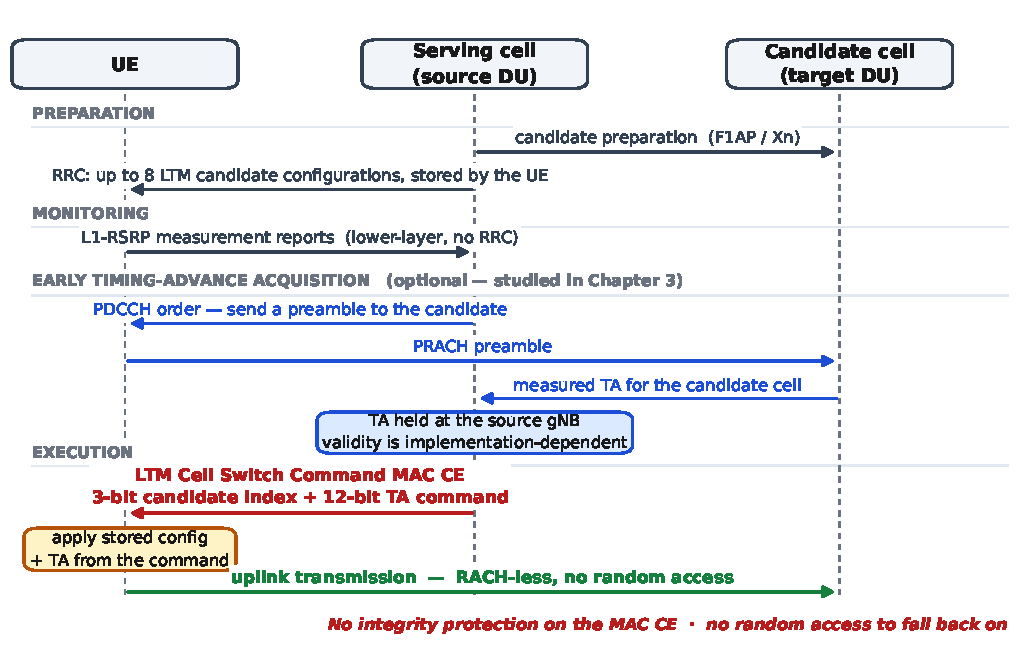
\includegraphics[width=\textwidth]{figures/ltm_flow.pdf}
  \caption{LTM procedure: preparation, monitoring, and execution. The optional early \TA{}
  acquisition phase pre-populates candidate \TA{} to enable RACH-less switching.}
  \label{fig:ltmflow}
\end{figure}

\begin{enumerate}\itemsep2pt
  \item \textbf{Preparation:} The serving gNB provisions up to eight candidate cell configurations
        to the UE via RRC. Configurations are pre-cached in UE memory, allowing subsequent switch
        commands to reference candidates via a compact 3-bit index.
  \item \textbf{Early Timing Advance Acquisition:} The network orders the UE to transmit a PRACH
        preamble to candidate cells prior to any handover~\cite{iqbal2024rachless}. The candidate DU
        measures the arrival delay,
        computes the \TA{}, and forwards it to the serving cell over F1AP. The basic \TA{} quantisation
        step is:
        \begin{equation}
          T_\mathrm{unit} = \frac{16 \cdot 64}{2^{\mu}}\, T_c ,
          \label{eq:taunit}
        \end{equation}
        evaluating to 520.8\,ns at $\mu=0$ (15\,kHz) and 260.4\,ns at $\mu=1$ (30\,kHz). One unit at
        $\mu=1$ corresponds to approximately 78\,m of one-way distance.
  \item \textbf{Execution (RACH-less):} When radio conditions warrant a switch, the serving cell transmits
        an LTM Cell Switch Command MAC CE containing the pre-calculated \TA{}. If a valid \TA{} is present,
        the UE skips the target cell RACH handshake and immediately commences transmission.
\end{enumerate}

\section{Related Work}

\paragraph{Handover and Low-Layer Attacks:}
Prior research demonstrates that cellular mobility procedures are vulnerable to unauthenticated inputs.
Shaik et al.~\cite{shaik2018rogue} demonstrated poisoning of self-organizing network (SON) handover
mechanisms. Bitsikas and Noubir~\cite{bitsikas2021donthandover} exposed vulnerabilities in unverified
RRC measurement reports. At layer~2, Erni et al.\ introduced AdaptOver~\cite{erni2022adaptover} and
5G-Overshadowing~\cite{erni20265gone}, showing that physical-layer signal overshadowing can reliably
inject unauthenticated MAC/RLC frames on commercial 5G networks. Luo et al.\ demonstrated SNI5GECT for
injection without a rogue base station~\cite{luo2025sni5gect}. Ludant et al.\ catalogued unprotected
low-layer control messages~\cite{ludant2025lowlayer} and demonstrated passive control sniffing via
5GSniffer~\cite{ludant2023sniffing}. Hamici-Aubert et al.~\cite{hamici2024overshadowing} forced RLC NACK
injections, inducing measurable transmission delays.

\paragraph{Scheduling Request Procedure Robustness:}
While low-layer scheduling and mobility procedures have been analyzed independently, no prior academic
study or 3GPP Change Request has investigated the interaction between the Scheduling Request retry
mechanism (TS~38.321 clause~5.4.4) and RACH-less LTM execution, searched via the 3GPP specification
change database and the academic literature cited in this section. \Cref{sec:m2gap} returns to this gap
with the decisive specification-level evidence that it is an omission rather than a deliberate design
choice.

\paragraph{Timing Advance Manipulation:}
\label{sec:lit-ta}
Kwao et al.~\cite{kwao2024random} demonstrated random access desynchronization attacks. Shanto, Karim,
and Bertino~\cite{shanto2026breaking} analyzed timing advance manipulation on commercial UEs, identifying
radio link failure (RLF) thresholds between 20 and 60 units. This figure is 3--10$\times$ larger than the
6--8 unit decodability boundary this report measures (\cref{sec:r1boundary}), but the two are not directly
comparable: Shanto et al.\ manipulate the \emph{serving} cell's actively closed-loop-tracked \TA{} and
measure \emph{RLF}, a downlink out-of-sync \emph{counter} that integrates over repeated measurement
intervals and is continuously nudged back toward correctness by the tracking loop between attacks; this
report instead measures the one-shot coded block-error rate of a single \emph{candidate}-cell uplink
transmission made with a \TA{} that was corrupted once, during early acquisition, and never
closed-loop-corrected before use. A UE tolerating a larger error before its serving-cell RLF counter
expires is accordingly not evidence that a freshly-applied, uncorrected candidate \TA{} would survive the
same error on its first transmission; reconciling the two thresholds on a common commercial receiver
remains open work, noted in \cref{sec:limits}.

\paragraph{MAC Control Element Security:}
Cao et al.~\cite{cao2025macce} surveyed MAC CE security broadly. Hätinen's 2026 study with
Ericsson~\cite{hatinen2026overshadowing} analyzed overshadowing across 69 MAC CEs. However, Hätinen's
analysis assumed that \TA{} corruption would be resolved by \texttt{timeAlignmentTimer} expiry and
subsequent RACH fallback. Crucially, that analysis pertained only to Conditional LTM (CLTM, clause
5.2), where a UE-side timer exists. Under plain LTM (clause 6.1.3.75), \TA{} is held by the network with
no UE-side timer and no fallback mechanism.

\paragraph{Handover Anomaly Detection:}
Dey and Patra~\cite{dey2025secure,dey2023handitover} proposed detecting handover DoS attacks in 5G-V2X
using machine learning classifiers trained on radio link failure and handover statistics.

\section{Research Gap}
\label{sec:gap}

Prior literature reveals two fundamental limitations:
\begin{enumerate}\itemsep2pt
  \item \textbf{Serving vs.\ Candidate Timing Advance:} Existing timing attacks target the serving cell,
        where closed-loop adjustments continuously correct drift, forcing an adversary to remain active.
        No prior work has examined candidate \TA{} values acquired in advance and stored asynchronously in
        network-side state without continuous closed-loop feedback.
  \item \textbf{Message Forgery vs.\ Architectural Logic:} Most low-layer security studies focus on
        exploiting the lack of MAC CE integrity protection via message forgery. Consequently, they do not
        investigate the protocol vulnerabilities created by LTM's speed-up architecture itself---specifically,
        how unauthenticated cached state interacts with disabled recovery procedures during RACH-less
        switching.
\end{enumerate}
This report bridges this gap by uncovering flaws in 3GPP specification logic that survive cryptographic
MAC CE integrity protection.

\chapter{Finding 1: Corrupted Early Timing Advance}
\label{ch:m1}

\section{Threat Model and Capabilities}
\label{sec:threat}

The adversary requires only two capabilities established in published literature and feasible with
commodity hardware:
\begin{enumerate}\itemsep2pt
  \item \textbf{Passive Downlink Sniffing:} The adversary decodes unencrypted physical-layer control
        information (DCI on PDCCH) using a passive receiver (e.g., 5GSniffer~\cite{ludant2023sniffing}).
        This reveals when an early PRACH transmission has been scheduled for a target candidate cell.
  \item \textbf{Radio-Frequency (RF) Relay:} The adversary captures the UE's PRACH preamble over the air
        and forwards it toward the candidate cell with an intentional propagation delay $\Delta$, without
        altering the preamble payload.
\end{enumerate}
The adversary possesses no cryptographic keys, cannot compromise gNB/UE internals, and does not forge
RRC messages. Crucially, this attack requires no forged MAC CEs, allowing it to survive future MAC CE
integrity protection.

\section{The Early Timing Advance Vulnerability}
\label{sec:m1attack}

Three architectural characteristics in 3GPP specifications enable the attack:

\subsection{Absence of Device-to-Preamble Binding}
When the serving gNB orders early \TA{} acquisition, the candidate cell is informed of three parameters:
the target cell ID, the assigned preamble index, and the PRACH occasion. It receives no cryptographic
token, UE identity (C-RNTI), or authentication tag. The candidate gNB correlates all incoming energy
in that occasion against the preamble sequence and extracts the timing offset corresponding to the
highest correlation peak. If an adversary forwards a delayed copy of the preamble with sufficient
power, the candidate cell accepts the delayed peak as legitimate, recording an inflated round-trip time.

\begin{figure}[htbp]
  \centering
  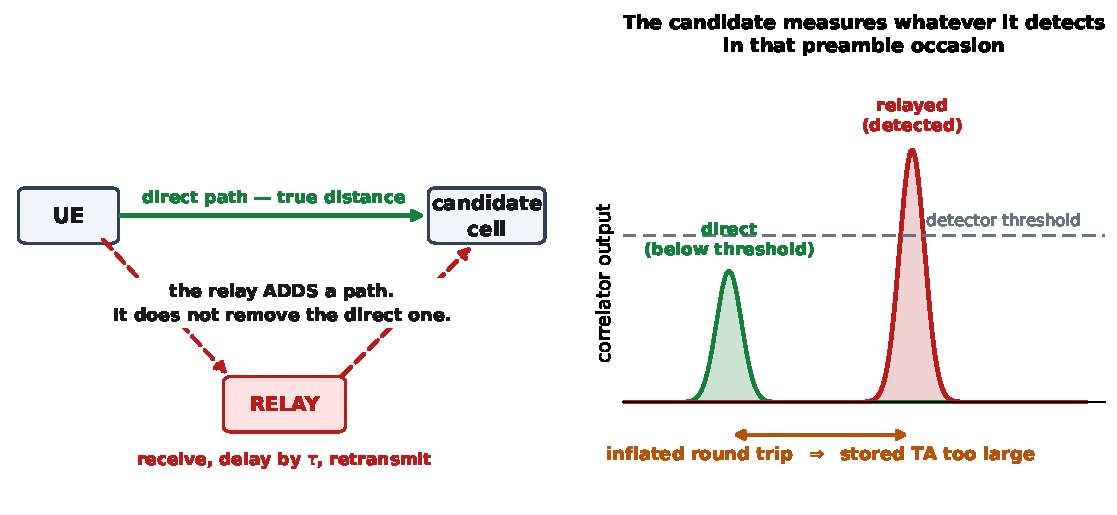
\includegraphics[width=\textwidth]{figures/atk05_relay.pdf}
  \caption{RF relay geometry. The candidate gNB correlates both the direct UE preamble and the
  delayed relayed copy. The attack succeeds when the relayed correlation peak exceeds the direct path.}
  \label{fig:relay}
\end{figure}

\subsection{Scope: Network-Supplied Candidate \TA{}}
\label{sec:m1scope}
Under TS~38.321 clause~5.2 and TS~38.213 clause~21~\cite{3gpp38213,3gpp38321}, an LTM switch obtains
its candidate \TA{} via one of two paths:
\begin{itemize}\itemsep2pt
  \item \textbf{Network-Supplied \TA{}:} The 12-bit Timing Advance Command in the LTM Cell Switch Command
        MAC CE contains an explicit integer value ($\ne \texttt{0xFFF}$). This value is populated by
        early acquisition.
  \item \textbf{UE-Measured \TA{}:} The Timing Advance Command is set to \texttt{0xFFF}, instructing the
        UE to reuse serving cell timing (applicable only to co-sited, synchronized candidates).
\end{itemize}
Our attack specifically targets the network-supplied path, which is universally required for inter-site
mobility across non-colocated base stations.

\subsection{Unbounded Network-Side Retention}
\label{sec:m1retention}
Once measured, the candidate \TA{} is transmitted across internal F1-C interfaces via the F1AP
\texttt{DU-CU TA INFORMATION TRANSFER} procedure~\cite{3gpp38473}. Remarkably, the F1AP Information
Element carries the cell ID, \TA{} value, preamble index, and RA-RNTI, but contains no timestamp,
sequence counter, or validity lifetime timer. TS~38.300 clause~9.2.3.5.2 states plainly that the UE does
not maintain a TA timer for the candidate cell, and that validity instead relies entirely on network
implementation~\cite{3gpp38300}. Because 3GPP specifies no retention limit, the serving cell may cache
this corrupted \TA{} indefinitely.
The adversary can execute the relay attack during an early preparation phase and depart; the damage is
only triggered when the network later issues the switch command.

\section{Theoretical Decodability Limit and Numerology Invariance}
\label{sec:m1boundary}

In 5G NR, the normal cyclic prefix duration is $L_{\mathrm{CP}} = 144 \cdot 64 \cdot T_c / 2^{\mu}$.
Dividing this by the basic timing advance unit $T_{\mathrm{unit}}$ from \cref{eq:taunit} yields:
\begin{equation}
  \frac{L_{\mathrm{CP}}}{T_{\mathrm{unit}}}
  = \frac{144 \cdot 64 \cdot T_c / 2^{\mu}}{16 \cdot 64 \cdot T_c / 2^{\mu}}
  = \frac{144}{16} = 9 \quad \text{\TA{} units, at all numerologies } \mu.
  \label{eq:cp9}
\end{equation}
The numerology scaling factor $2^{-\mu}$ cancels identically. Consequently, the theoretical cyclic prefix
guard interval spans exactly $9\,T_{\mathrm{unit}}$ regardless of subcarrier spacing ($\mu \in \{0, 1, 2, 3\}$).
In real propagation channels, multipath delay spread consumes a fraction of this guard interval; the exact
empirical failure cliff under realistic channel models is evaluated experimentally in \cref{ch:results}.

\section{Relay Feasibility and Link-Budget Geometry}
\label{sec:m1delay}

For the relay's forwarded signal to capture the candidate gNB's PRACH correlator, its received power at
the gNB must exceed the direct UE path by a threshold $\Delta_{\mathrm{th}}$:
\begin{equation}
  \underbrace{(P_{\mathrm{relay}} - P_{\mathrm{UE}})}_{\text{Power Advantage}}
  - \underbrace{\bigl(\mathrm{PL}(r) - \mathrm{PL}(d)\bigr)}_{\text{Path-Loss Disadvantage}}
  \;\ge\; \Delta_{\mathrm{th}} ,
  \label{eq:linkbudget}
\end{equation}
where $d$ is the candidate-to-UE distance, $r$ is the candidate-to-relay distance, and $\mathrm{PL}(\cdot)$
is path loss in dB modeled via 3GPP TR~38.901~\cite{3gpp38901}. Throughout this section, $\Delta_{\mathrm{th}}$
is not an assumed constant: it is the empirical 90\% capture threshold established experimentally via
srsRAN simulation in \cref{sec:r1capture} ($+9.9$\,dB under flat fading, $+5.3$\,dB under urban multipath),
substituted here to project relay feasibility over distance and power.

\begin{table}[htbp]
  \centering
  \caption{Maximum allowable candidate-to-relay distance $r$ achieving 90\% capture threshold
  ($\Delta_{\mathrm{th}} = +9.9$\,dB for flat fading; $+5.3$\,dB for urban multipath), 3.5\,GHz UMa NLOS,
  at two representative macro-cell victim distances. The ratio $r/d$ is distance-invariant (confirmed
  across 200\,m--2\,km in \cref{fig:capture}, right panel), so only $d=500$\,m and $d=1000$\,m are shown
  here; the same ratios apply at any $d$.
  Analytic projection from the TR~38.901 path-loss model (\cref{eq:linkbudget}), not a Monte Carlo
  measurement.}
  \label{tab:link}
  \small
  \begin{tabular}{@{}lrr@{}}
    \toprule
    Relay Power Advantage & $d=500$\,m & $d=1000$\,m \\
    \midrule
    \multicolumn{3}{@{}l}{\emph{Flat Rayleigh Fading ($\Delta_{\mathrm{th}} = +9.9$\,dB)}} \\
    $0$\,dB (23\,dBm)   & 275\,m  & 555\,m  \\
    $+10$\,dB (33\,dBm) & 500\,m  & 1005\,m \\
    $+20$\,dB (43\,dBm) & 905\,m  & 1810\,m \\
    \addlinespace
    \multicolumn{3}{@{}l}{\emph{Urban Multipath Profile ($\Delta_{\mathrm{th}} = +5.3$\,dB)}} \\
    $0$\,dB (23\,dBm)   & 365\,m  & 730\,m  \\
    $+10$\,dB (33\,dBm) & 655\,m  & 1315\,m \\
    $+20$\,dB (43\,dBm) & 1185\,m & 2375\,m \\
    \bottomrule
  \end{tabular}
\end{table}

As shown in \cref{tab:link}, a relay radiating 33\,dBm (a modest 10\,dB advantage over a standard 23\,dBm
handset) achieves capture from any location where $r \le d$. Under urban multipath, the required margin
drops to 5.3\,dB, expanding the operational zone to $r \le 1.3\,d$. Thus, the attacker faces no delicate
positioning constraints.

Furthermore, an induced delay of seven units at $\mu=1$ corresponds to $7 \times 260.4\,\text{ns} = 1.82\,\mu\text{s}$,
equivalent to an excess propagation path of $547$\,m. An adversary can introduce this delay entirely
geometrically by positioning itself off the direct line-of-sight path between the UE and the candidate cell.

\section{Analysis of Network-Controlled Repeaters (NCR)}
\label{sec:m1ncr}

3GPP Release 18 standardized Network-Controlled Repeaters (NCR) as low-cost coverage
extenders~\cite{3gpp38867,carvalho2024ncr}.
Because repeaters introduce group delay, it is essential to determine whether deployed repeaters already
induce this failure accidentally, or whether an active adversary is required.

\begin{table}[htbp]
  \centering
  \caption{Forwarding delay of relay/repeater technologies at $\mu=1$ ($260.4$\,ns per \TA{} unit). The
  SDR figure is the receive-path latency reported directly in~\cite{usrplatency} (not a derived or
  halved round-trip estimate).}
  \label{tab:hardware}
  \small
  \begin{tabularx}{\textwidth}{@{}l r r X@{}}
    \toprule
    Hardware Type & Latency & \TA{} Units & Impact on Attack Feasibility \\
    \midrule
    Host-controlled SDR~\cite{usrplatency} & 57.6--126\,$\mu$s & 221--484 & Exceeds PRACH search window \\
    FPGA loopback relay~\cite{nifpgaloopback} & 550\,ns & 2.1 & Requires buffer to reach 7 units \\
    Commercial digital repeater~\cite{ti2018repeater} & 2--6\,$\mu$s & 7.7--23.0 & Readily exceeds 7 units \\
    3GPP Release-18 NCR~\cite{3gpp38867,carvalho2024ncr} & tens of ns & $\sim$0.1 & Negligible delay; fails harmlessly \\
    \bottomrule
  \end{tabularx}
\end{table}

As shown in \cref{tab:hardware}, standardized 3GPP NCRs operate with analog RF filtering latencies under
50\,ns (consuming $<0.2\,T_{\mathrm{unit}}$), which is harmless. Furthermore, in legacy networks, repeater
propagation delays are \textbf{common-mode}: because the same physical path is used during both RACH
estimation and subsequent data transmission, static delays cancel out naturally.

Early acquisition breaks this common-mode cancellation. The \TA{} is measured across one path (e.g.,
through an adversary's relay), stored indefinitely, and subsequently applied across a different path
during RACH-less handover. What an adversary supplies is not absolute delay, but \textbf{differential
delay} that is frozen into network state.

\chapter{Finding 2: Scheduling Request Deadlock}
\label{ch:m2}

\section{The Scheduling Request Procedure in TS 38.321}
\label{sec:m2proc}

In 5G NR, a UE requires an explicit uplink grant from the gNB before transmitting on the Physical Uplink
Shared Channel (PUSCH). In a legacy handover, the UE executes the Random Access (RACH) procedure; the
gNB responds with Msg2 (Random Access Response), which explicitly provides both uplink timing alignment
and an initial uplink grant.

In contrast, RACH-less LTM intentionally skips the random access handshake. Under TS~38.300
clause~9.2.3.5.1, the UE accesses the target cell via either a configured grant or a dynamic grant, and
begins monitoring PDCCH on the target cell for dynamic scheduling as soon as the switch starts; it may
not trigger random access before the switch completes unless it holds a valid PUCCH resource for the
SR. When dynamic grant scheduling is used, the cell switch command MAC CE can additionally carry an SR
configuration ID pointing the UE to the PUCCH resource for sending that request~\cite{3gpp38300}.
Because pre-allocating dedicated configured grants across all candidate cells is resource-intensive and
optional, standard deployments rely on dynamic scheduling. The UE arrives at the target cell with
no valid uplink grant, forcing it to issue a Scheduling Request (SR)---a 1-bit indicator on
PUCCH Format~0---to request an initial grant to transmit its \texttt{RRCReconfigurationComplete} message.

TS~38.321 clause~5.4.4 governs the SR retry loop~\cite{3gpp38321}. The UE maintains an internal counter
\texttt{SR\_COUNTER}, initialized to zero. For each transmission attempt, the UE increments \texttt{SR\_COUNTER}
and starts \texttt{sr-ProhibitTimer}. If an uplink grant arrives, the procedure terminates successfully.
However, if no grant is received after \texttt{sr-TransMax} attempts, \texttt{SR\_COUNTER} exhausts and
execution falls into the clause's \texttt{else} branch.

\section{The Specification Defect: TS 38.321 Clause 5.4.4}
\label{sec:m2gap}

\Cref{fig:deadlock} illustrates TS~38.321 clause~5.4.4 as a formal condition tree, preserving 3GPP's
normative indentation depths (\texttt{1>} through \texttt{6>}). A critical structural defect exists
in the asymmetric placement of resource teardown versus recovery actions:

\begin{figure}[htbp]
  \centering
  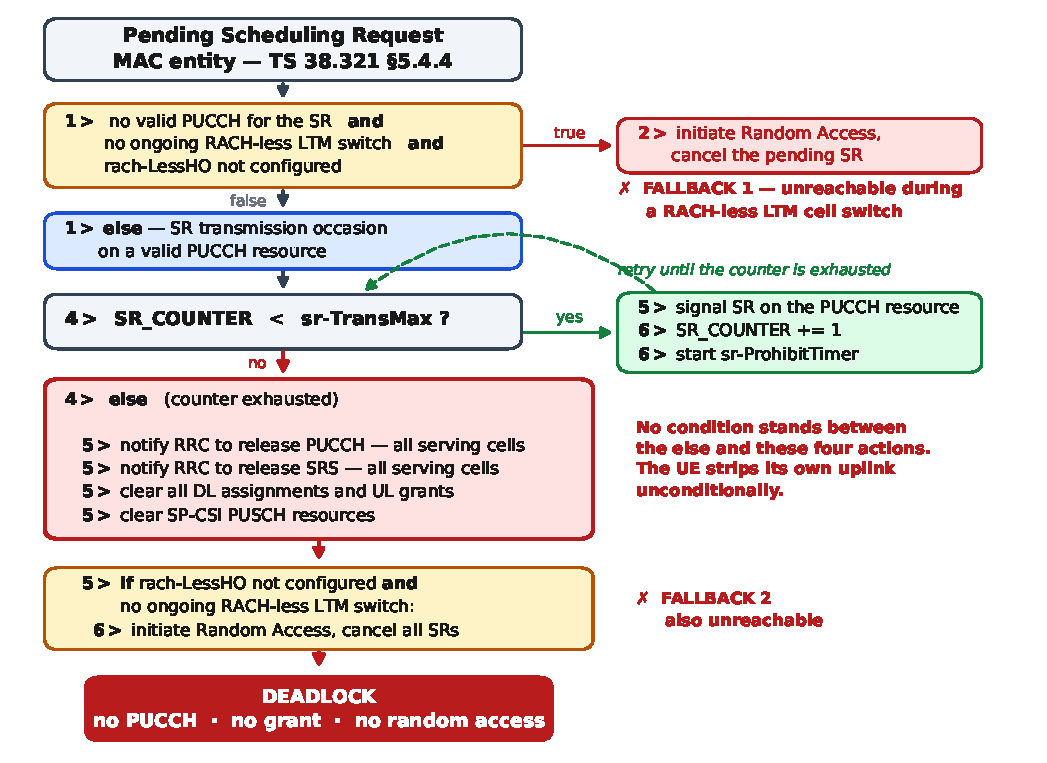
\includegraphics[width=\textwidth]{figures/atk16_deadlock.pdf}
  \caption{Condition tree of TS~38.321 clause~5.4.4. The resource deallocation actions at depth \texttt{5>}
  execute unconditionally on counter exhaustion. The recovery action (initiating Random Access) at depth
  \texttt{6>} is blocked because the guard condition evaluates to false during a RACH-less LTM switch.}
  \label{fig:deadlock}
\end{figure}

\begin{itemize}\itemsep2pt
  \item \textbf{Unconditional Resource Teardown (Depth \texttt{5>}):} When \texttt{SR\_COUNTER} exhausts,
        the specification executes four destructive actions directly beneath the \texttt{else} statement
        with no qualifying conditions, unconditionally stripping the UE of all physical uplink control and
        grant resources: release of PUCCH and SRS for all serving cells, clearing of all configured
        downlink assignments and uplink grants, and clearing of any PUSCH resource for semi-persistent CSI
        reporting---including the very PUCCH channel used to signal scheduling requests.
  \item \textbf{Gated Recovery Path (Depth \texttt{6>}):} The sole action that would restore uplink
        connectivity---initiating random access to recover from the failure---is nested one level deeper,
        conditioned on \texttt{rach-LessHO} being unconfigured and no RACH-less LTM cell switch being
        ongoing; only then does the UE initiate Random Access (clause~5.1) on the SpCell and cancel all
        pending SRs.
\end{itemize}

During an ongoing RACH-less LTM switch, the second conjunct is \textbf{false}. Consequently, the recovery
action at depth \texttt{6>} is completely skipped. Furthermore, the clause's alternative path to random
access (taken if no valid PUCCH resource is configured) is guarded by the identical condition.

\paragraph{Protocol Deadlock:} The UE loses every UE-initiated path back to uplink connectivity:
\begin{enumerate}\itemsep1pt
  \item It holds no uplink grants and no PUCCH resources to request new grants.
  \item The only mechanism capable of allocating new resources on its own initiative (Random Access) is
        explicitly forbidden.
  \item The blocking condition, an ongoing RACH-less LTM cell switch, cannot clear, because cell-switch
        completion requires transmitting an RRC reconfiguration complete message, which is impossible
        without an uplink grant.
\end{enumerate}
The same clause~9.2.3.5.1 keeps the UE monitoring PDCCH for a dynamic grant throughout
(\cref{sec:m2proc}), so the bare defect is not strictly permanent on its own; \cref{sec:m2dyngrant} shows
why the attack closes that escape anyway.

\section{The Attack: Forcing Deadlock via Corrupted Timing Advance}
\label{sec:m2threat}

While the deadlock defect exists as an inherent specification flaw, reaching counter exhaustion by chance
under normal radio conditions is vanishingly rare ($P \approx 10^{-12}$). However, an adversary leverages
the corrupted candidate \TA{} from Finding~1 to drive the UE into this deadlock deterministically.

\subsection{Attack Execution}
The attack proceeds in five deterministic steps:
\begin{enumerate}\itemsep2pt
  \item \textbf{Preamble Delay Injection:} During candidate cell early acquisition, the adversary's RF
        relay intercepts the UE's preamble and forwards it with $\Delta \ge 7\,T_{\mathrm{unit}}$ excess
        delay. The candidate gNB computes an inflated \TA{} and forwards it to the serving gNB via F1AP.
  \item \textbf{RACH-less Handover Trigger:} The serving gNB issues an LTM Cell Switch Command MAC CE
        containing this corrupted \TA{}. Because a \TA{} is present, TS~38.300 mandates a RACH-less switch.
        The UE applies the bad \TA{} and skips random access.
  \item \textbf{PUCCH SR Decorrelation:} Arriving at the target cell with no grant, the UE transmits an
        SR on the PUCCH resource indicated by the switch command. Because its transmit timing is
        misaligned by $\ge 7\,T_{\mathrm{unit}}$, the gNB detector's coherent phase correlation across
        subcarriers collapses completely. The target gNB cannot decode the SR.
  \item \textbf{Deterministic Counter Exhaustion:} The UE retransmits the SR at every periodic occasion.
        Because the timing error is static and persistent, every subsequent SR attempt fails with high
        probability. \texttt{SR\_COUNTER} reaches \texttt{sr-TransMax} with near certainty under flat
        fading ($P \ge 0.996$ at 7 units) and with high probability under multipath ($P = 0.75$--$0.97$,
        \cref{tab:determinism}).
  \item \textbf{Deadlock:} Clause 5.4.4 executes the \texttt{else} branch, releasing PUCCH, SRS, and all
        grants. Because the switch is RACH-less, random access is blocked. The UE is silenced; whether it
        stays silenced is addressed in \cref{sec:m2dyngrant}.
\end{enumerate}

\begin{table}[htbp]
  \centering
  \caption{Comparison of SR counter exhaustion by random channel fading versus corrupted \TA{} attack
  at $\texttt{sr-TransMax}=8$, 10\,dB SNR, 1 receive port.}
  \label{tab:determinism}
  \small
  \begin{tabularx}{\textwidth}{@{}l X r r@{}}
    \toprule
    Timing Condition & Channel Environment & Per-Attempt Loss & $P(\text{Exhaustion})$ \\
    \midrule
    \multicolumn{4}{@{}l}{\textbf{Honest UE (Aligned \TA{})}} \\
    Synchronized ($\Delta_{\mathrm{TA}} = 0$) & Flat Rayleigh fading & 0.0365 & $3.0 \times 10^{-12}$ \\
    Synchronized ($\Delta_{\mathrm{TA}} = 0$) & Additive White Gaussian Noise & $<0.0005$ & $\ll 10^{-9}$ \\
    \midrule
    \multicolumn{4}{@{}l}{\textbf{Adversary-Corrupted \TA{} Attack}} \\
    Error $\Delta_{\mathrm{TA}} = 6$ units & Flat Rayleigh fading & 0.9720 & $0.797$ \\
    Error $\Delta_{\mathrm{TA}} = 7$ units & Flat Rayleigh fading & 0.9995 & $0.996$ \\
    Error $\Delta_{\mathrm{TA}} = 7$ units & Urban Multipath Profile & 0.9650 & $0.750$ \\
    Error $\Delta_{\mathrm{TA}} = 8$ units & Urban Multipath Profile & 0.9965 & $0.970$ \\
    Error $\Delta_{\mathrm{TA}} \ge 8$ units & AWGN / Flat fading & 1.0000 & $1.000$ \\
    \bottomrule
  \end{tabularx}
\end{table}

\subsection{Why the Trigger is Deterministic}
As shown in \cref{tab:determinism}, random channel errors result in independent Bernoulli trials,
yielding an exhaustion probability of $0.0365^8 \approx 3 \times 10^{-12}$. In contrast, a timing
advance error of $\ge 7$ units creates correlated, structural failures: every transmission
arrives misaligned. The per-attempt loss probability reaches $0.9995$, driving the probability of
deadlock to $0.996$ under flat fading and $0.970$ under multipath (at 8 units).

\subsection{The Dynamic Grant Does Not Save the UE}
\label{sec:m2dyngrant}
TS~38.300 clause~9.2.3.5.1 lets the gNB schedule the UE on PDCCH without waiting for an SR, so the bare
specification defect is not, by itself, permanent---a grant the UE never requested would still restore
it. Under the attack, this escape closes twice over. First, any grant the gNB issues still has to be
used on the same misaligned uplink timing: a PUSCH transmission suffers the identical $\ge 7$-unit
offset as the SR did, so it is no more decodable than the request that triggered it. Second, the gNB
has no reason to issue a grant in the first place: it has received nothing from this UE since the
switch began, and an SR-silenced UE is, from the network's side, indistinguishable from an idle one
that has nothing to send. The deadlock is therefore not unbreakable in principle, but the same
corruption that causes it also removes the one practical way out.

\section{Formal Model of Counter Exhaustion and Parameter Space Sweep}
\label{sec:m2model}

Reaching deadlock depends on a race between the time required to exhaust \texttt{SR\_COUNTER}
($T_{\text{exhaust}}$) and the mobility supervision timer \texttt{t304}. The time to exhaustion is:
\begin{equation}
  T_{\text{exhaust}} = \texttt{sr-TransMax} \times T_{\text{interval}},
  \quad
  T_{\text{interval}} = \max\!\left(P_{\mathrm{ms}},\
    \left\lceil \frac{\texttt{sr-ProhibitTimer}}{P_{\mathrm{ms}}} \right\rceil P_{\mathrm{ms}} \right),
  \label{eq:exhaust}
\end{equation}
where $P_{\mathrm{ms}} = P / 2^{\mu}$ represents the SR resource periodicity in milliseconds, and
$T_{\text{interval}}$ accounts for the quantization of \texttt{sr-ProhibitTimer} onto available SR occasions.

\paragraph{State Transition and Deadlock Logic of TS~38.321 Clause~5.4.4:}
The procedural flow of the MAC entity upon SR counter exhaustion proceeds as follows:
\begin{enumerate}\itemsep1pt
  \item \textbf{Periodic Transmission Phase:} At each valid SR occasion spaced by $T_{\text{interval}}$ (\cref{eq:exhaust}), the UE transmits an SR on PUCCH Format~0 and increments \texttt{SR\_COUNTER}.
  \item \textbf{Supervision Timer Race:} If the handover supervision timer \texttt{t304} expires before \texttt{SR\_COUNTER} reaches \texttt{sr-TransMax} ($t \ge \texttt{t304}$), the UE declares handover failure and initiates standard RRC connection re-establishment.
  \item \textbf{Unconditional Teardown (Depth 5>):} When $\texttt{SR\_COUNTER} \ge \texttt{sr-TransMax}$, the MAC entity unconditionally executes:
    \begin{itemize}\itemsep0pt
      \item Notify RRC to release PUCCH and SRS for all serving cells;
      \item Clear any configured downlink assignments and uplink grants;
      \item Clear any semi-persistent CSI reporting resources.
    \end{itemize}
  \item \textbf{Recovery Evaluation (Depth 6>):} The MAC entity evaluates the guard condition for recovery:
    \begin{itemize}\itemsep0pt
      \item \textbf{Legacy / Non-LTM Handover:} If \texttt{rach-LessHO} is not configured, the condition evaluates to true; the UE initiates a Random Access procedure on the target cell to recover.
      \item \textbf{RACH-less LTM Switch:} Because an ongoing RACH-less LTM switch is active, the guard condition strictly evaluates to false. The UE is forbidden from initiating Random Access.
    \end{itemize}
  \item \textbf{Protocol Deadlock State:} With all uplink transmission resources torn down and Random Access recovery inhibited, the UE has no remaining UE-initiated path back to uplink connectivity and is silenced for the remaining duration $T_{\text{dead}} = \texttt{t304} - T_{\text{exhaust}}$, until \texttt{t304} eventually expires. A network-issued dynamic grant remains possible on paper (\cref{sec:m2proc}); \cref{sec:m2dyngrant} shows why it does not materialize in practice, making the dead state effectively unbreakable until timeout.
\end{enumerate}

\subsection{Parameter Space Enumeration (5400 Configurations)}
\label{sec:m2space}
3GPP specifications define parameters via formal ASN.1 definitions in TS~38.331~\cite{3gpp38331}:
\begin{itemize}\itemsep1pt
  \item \texttt{sr-TransMax}: 5 legal values ($\{n4, n8, n16, n32, n64\}$).
  \item \texttt{sr-ProhibitTimer}: 18 legal values (8 Rel-15 values, absent $=0$, plus 9 Rel-17 values).
  \item SR periodicity $P$: 15 legal values ($\{sym2, sym7, sl1, sl2, sl4, \dots, sl640\}$).
  \item Numerology $\mu$: 4 values ($\mu \in \{0, 1, 2, 3\}$).
\end{itemize}
This establishes a finite space of $5 \times 18 \times 15 \times 4 = 5400$ valid 3GPP configurations.
Evaluating this state transition logic across all 5400 configurations reveals that when no LTM switch is ongoing, 100\%
of configurations safely recover via random access. However, during a RACH-less LTM switch, between
\textbf{9.0\% and 77.4\%} of configurations reach this effectively-unbreakable dead state (\cref{sec:m2dyngrant}).

\section{Outage Cost and Timer Interaction}
\label{sec:m2cost}

When deadlock occurs, the UE remains silenced for an outage duration
$T_{\text{dead}} = \texttt{t304} - T_{\text{exhaust}}$ until the supervision timer \texttt{t304} expires.
During $T_{\text{dead}}$, the UE can neither transmit data nor request resources.

\paragraph{Why Radio Link Failure (T310) Does Not Intervene:} One might expect the radio link failure
timer T310 to rescue the UE. It cannot, for two reasons: (i) T310 monitors downlink PDCCH block
error rate, which remains healthy; and (ii) TS~38.331 clause~5.3.5.4 mandates that applying the
\texttt{ReconfigurationWithSync} information element (which starts T304) explicitly stops T310.

\paragraph{Evidence from Clause 5.2 (Conditional LTM Comparison):}
The decisive proof that this defect represents a specification omission appears in TS~38.321 clause~5.2
(governing \texttt{timeAlignmentTimer} expiry)~\cite{3gpp38321}: when a RACH-less CLTM cell switch is
ongoing, the clause branches to initiate Random Access (clause~5.1) on the SpCell; only its \texttt{else}
branch releases PUCCH and SRS and clears grants without that escape. 3GPP therefore already recognized
that a UE losing resources during a RACH-less switch requires an escape to random access, and added it
for Conditional LTM. However, 3GPP omitted this identical remedy from clause~5.4.4 for plain LTM.
Re-inserting this escape into clause~5.4.4 forms the core of our proposed 3GPP remediation.

\chapter{Results, Validation and Discussion}
\label{ch:results}

\section{Physical-Layer Preamble Capture (Finding 1)}
\label{sec:r1capture}

Using the srsRAN 5G physical-layer implementation~\cite{srsran} under 3GPP TR~38.901 channel models,
we evaluated the relative relay power advantage required to capture the candidate gNB's PRACH correlator.
The simulation executed 2000 Monte Carlo trials per configuration at 30\,kHz ($\mu=1$) with preamble
format~B4.

\begin{table}[htbp]
  \centering
  \caption{Relay received power advantage relative to direct UE path required to capture the candidate cell
  correlator (2000 trials per point), shown for three representative delays spanning the full swept range
  7--32 units; the threshold is delay-invariant, as the near-identical rows below confirm.}
  \label{tab:capture}
  \small
  \begin{tabular}{@{}c rrrr@{}}
    \toprule
    Relay Delay $\Delta$ & \multicolumn{2}{c}{Flat Rayleigh Fading} & \multicolumn{2}{c}{20-Tap Urban Multipath} \\
    \cmidrule(lr){2-3} \cmidrule(lr){4-5}
    ($T_{\mathrm{unit}}$) & 50\% Capture & 90\% Capture & 50\% Capture & 90\% Capture \\
    \midrule
    7  & $+0.23$\,dB & $+9.89$\,dB & $+0.05$\,dB & $+5.53$\,dB \\
    16 & $+0.21$\,dB & $+9.87$\,dB & $+0.09$\,dB & $+5.31$\,dB \\
    32 & $+0.22$\,dB & $+9.88$\,dB & $+0.06$\,dB & $+5.32$\,dB \\
    \bottomrule
  \end{tabular}
\end{table}

\begin{figure}[htbp]
  \centering
  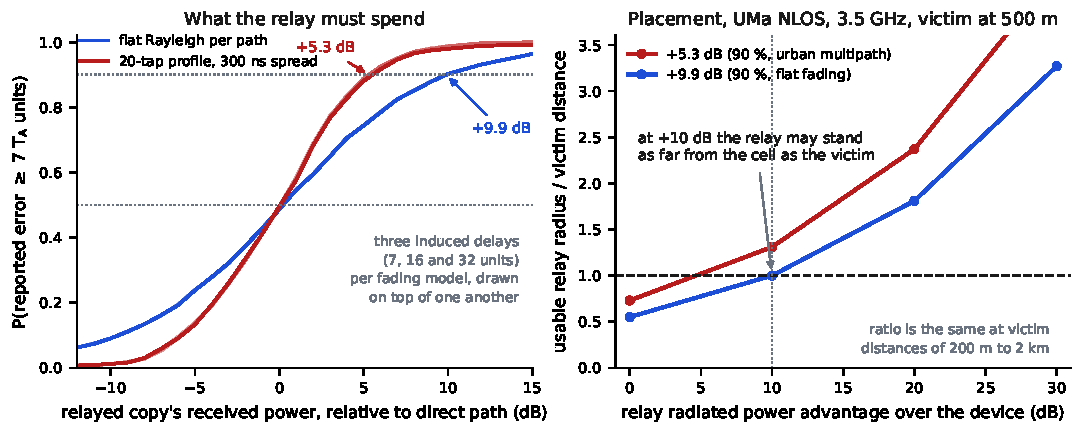
\includegraphics[width=\textwidth]{figures/atk05a_capture.pdf}
  \caption{Left: Preamble capture probability versus relay power advantage. Right: Admissible relay
  operating radius normalized by victim distance under TR~38.901 path loss.}
  \label{fig:capture}
\end{figure}

As shown in \cref{tab:capture} and \cref{fig:capture}, three critical properties emerge:
\begin{enumerate}\itemsep1pt
  \item \textbf{Delay-Invariant Power Threshold:} The 90\% capture threshold remains constant at $+9.9$\,dB
        under flat fading across all injected delays (7 to 32 units). The PRACH correlation sequence has
        a flat frequency spectrum; thus, the correlator contest is decided strictly by relative received
        amplitude rather than temporal displacement.
  \item \textbf{Multipath Reduces Attacker Cost:} Under realistic 20-tap urban multipath (300\,ns delay
        spread), the required 90\% power advantage drops by 4.6\,dB to $+5.3$\,dB. Multipath disperses
        preamble energy into reflection clusters, increasing the probability that a relayed multipath tap
        produces the dominant correlation peak.
  \item \textbf{Geographic Feasibility:} Under TR~38.901 urban path loss, a $+10$\,dB power advantage
        permits the relay to operate anywhere within a radius $r \le d$ from the candidate cell,
        confirming that the attacker faces no delicate spatial positioning constraints.
\end{enumerate}

\section{Decodability Boundary and Receiver Retracking}
\label{sec:r1boundary}

To determine the exact point where timing misalignment destroys uplink reception, we evaluated the
OpenAirInterface (OAI)~\cite{oai} LDPC coding chain under time-domain timing offsets. Link failure is
defined as coded $\text{BLER} \ge 0.99$.

While the theoretical cyclic prefix guard interval spans 9 units (\cref{eq:cp9}), channel delay spread
and receiver filtering consume part of this budget in practice. The empirical decodability boundary in
the early transmission direction spans \textbf{6 to 8 units (median 7 units)}, corresponding to
$1.82\,\mu\text{s}$ at 30\,kHz. Beyond 12 units, post-equalization SNR drops below $-24$\,dB across all
modulation orders (QPSK through 256-QAM) and code rates (0.19 to 0.66).

\begin{figure}[htbp]
  \centering
  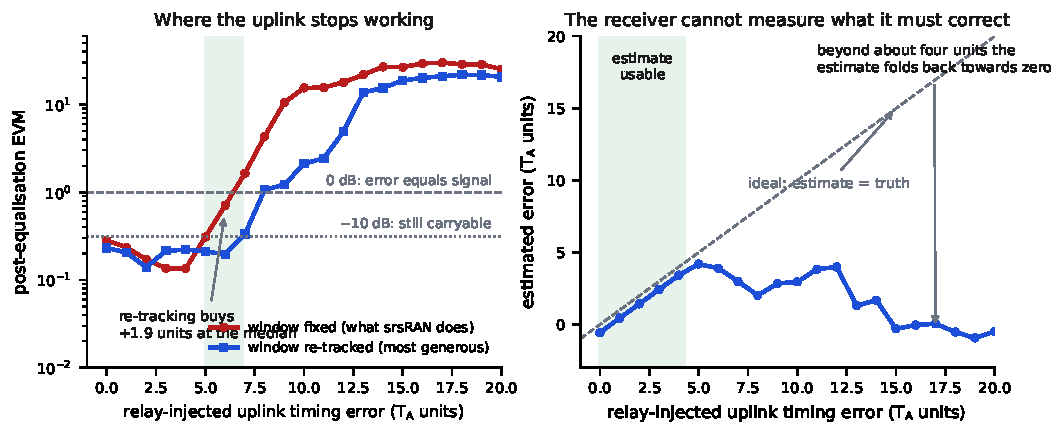
\includegraphics[width=\textwidth]{figures/atk05b_retrack.pdf}
  \caption{Left: Post-equalization EVM versus timing error before and after receiver tracking. Right:
  Receiver timing estimation error, exhibiting foldback towards zero beyond 4 units.}
  \label{fig:retrack}
\end{figure}

\paragraph{Failure of Receiver Re-tracking:} Modern 5G base stations employ digital tracking loops to track
sub-microsecond timing drift from mobile UEs. We evaluated whether this tracking mechanism could detect
a 7-unit error and shift its receiver FFT window to rescue the connection. As shown in \cref{fig:retrack},
closed-loop tracking provides a maximum correction of only $+4.38$ units (median $+1.86$), beyond which
phase ambiguity causes the estimator to fold back toward zero rather than continue tracking the true
error. At 7 units of true error, the receiver tracking loop is ineffective and cannot detect or correct
the error.

\section[Window Confinement Mitigation (ZCZ)]{Window Confinement Mitigation via ZCZ Search Window}
\label{sec:r1zcz}

The gNB PRACH search window is governed by \texttt{zeroCorrelationZoneConfig} (ZCZ), which sets the
cyclic shift $N_{\mathrm{CS}}$. A correlator cannot report delays exceeding its search window.

\begin{table}[htbp]
  \centering
  \caption{PRACH search window and damaging error probability by ZCZ configuration (2000 trials).}
  \label{tab:zcz}
  \small
  \begin{tabular}{@{}c r rrr@{}}
    \toprule
    ZCZ & Window & \multicolumn{3}{c}{$P(\text{Damaging Error})$} \\
    \cmidrule(lr){3-5}
    Index & ($T_{\mathrm{unit}}$) & $0$\,dB & $+3$\,dB & $+6$\,dB \\
    \midrule
    \multicolumn{5}{@{}l}{\emph{Safe Configurations (Search Window $< 7\,T_{\mathrm{unit}}$)}} \\
    1  & 0.40  & 0.000 & 0.000 & 0.000 \\
    2  & 2.00  & 0.000 & 0.000 & 0.000 \\
    3  & 3.60  & 0.000 & 0.000 & 0.000 \\
    4  & 4.80  & 0.000 & 0.000 & 0.000 \\
    5  & 6.40  & 0.000 & 0.000 & 0.000 \\
    \midrule
    \multicolumn{5}{@{}l}{\emph{Exposed Configurations (Search Window $\ge 7\,T_{\mathrm{unit}}$)}} \\
    8  & 10.00 & 0.886 & 0.931 & 0.967 \\
    9  & 11.60 & 0.986 & 0.994 & 0.996 \\
    10 & 13.20 & 1.000 & 1.000 & 1.000 \\
    12 & 18.80 & 0.718 & 0.836 & 0.909 \\
    15 & 46.40 & 0.487 & 0.650 & 0.786 \\
    \bottomrule
  \end{tabular}
\end{table}

As shown in \cref{tab:zcz}, configurations 1 through 5 constrain the searchable delay below the 7-unit
decodability boundary, completely eliminating damaging errors ($P=0$). However, this protection trades
directly against cell radius: ZCZ configurations $\le 5$ limit maximum cell radius to under 500\,m,
making them unusable in macro-cell deployments.

\section{Scheduling Request Failure Under Corrupted Timing Advance}
\label{sec:r2sr}

Next, we evaluate the decodability of PUCCH Format~0 Scheduling Requests under timing errors. We evaluated
srsRAN's physical-layer Format~0 detector across 2000 trials per point.

\begin{figure}[htbp]
  \centering
  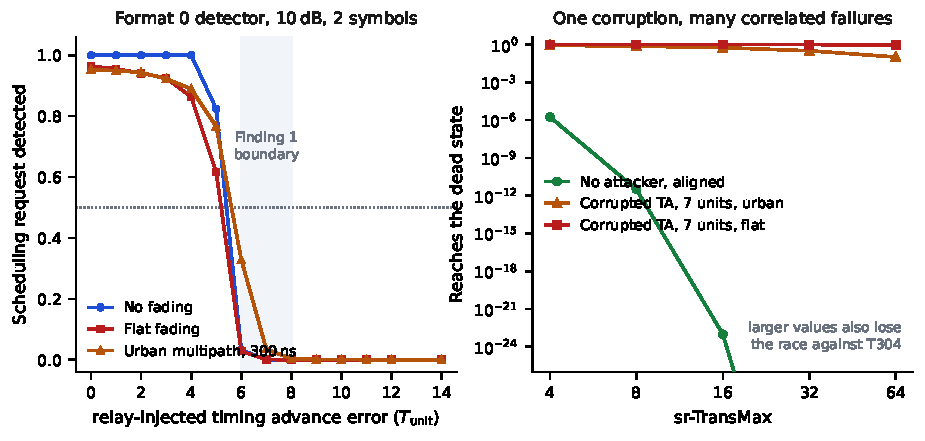
\includegraphics[width=\textwidth]{figures/atk16_sr.pdf}
  \caption{Left: PUCCH Format~0 SR recovery probability versus \TA{} error across channel models.
  Right: Deterministic escalation to counter exhaustion ($P > 0.99$) under 7 units of \TA{} error.}
  \label{fig:sr}
\end{figure}

\paragraph{Analytical Coherence Collapse:} PUCCH Format~0 transmits a single bit via a cyclic shift of a
base sequence across the 12 subcarriers of one resource block. An uncompensated timing offset introduces
an escalating phase rotation across the subcarriers ($e^{-j 2\pi k \Delta f \tau}$), causing destructive
phase cancellation during coherent receiver correlation. Consequently, the correlation peak drops below
the gNB's detection threshold ($0.5273$ in srsRAN) by 6 to 7 units of error, as confirmed by our
simulations in \cref{tab:srports}.

\begin{table}[htbp]
  \centering
  \caption{PUCCH Format~0 SR detection probability versus receive antenna ports and timing error
  (Flat Rayleigh fading, 10\,dB SNR, 2000 trials).}
  \label{tab:srports}
  \small
  \begin{tabular}{@{}l rrrrrr@{}}
    \toprule
    Receive Ports & Threshold & 0 units & 5 units & 6 units & 7 units & 8 units \\
    \midrule
    1 Port  & 0.5273 & 0.964 & 0.616 & 0.028 & 0.0005 & \textbf{0.000} \\
    2 Ports & 0.3455 & 0.998 & 0.968 & 0.432 & 0.0010 & \textbf{0.000} \\
    4 Ports & 0.2545 & 1.000 & 1.000 & 0.955 & 0.0205 & \textbf{0.000} \\
    \bottomrule
  \end{tabular}
\end{table}

\paragraph{Simulation Verification:} As shown in \cref{fig:sr} and \cref{tab:srports}, SR detection
collapses abruptly between 5 and 7 units. At 7 units of error, SR recovery probability is $0.0005$ at
1 port and $0.0205$ at 4 ports. At 8 units of error, not a single SR is detected in 2000 trials across
any antenna configuration. Because the failure is caused by phase decorrelation rather than noise,
increasing SNR from $-3$\,dB to $+20$\,dB yields 0\% recovery. The target gNB is blind to the request.

\section{Parameter Space Sweep and Outage Evaluation}
\label{sec:r2}

We evaluated the complete 5400-configuration space defined in \cref{sec:m2model} across varying handover
supervision windows (\texttt{t304}).

\begin{figure}[htbp]
  \centering
  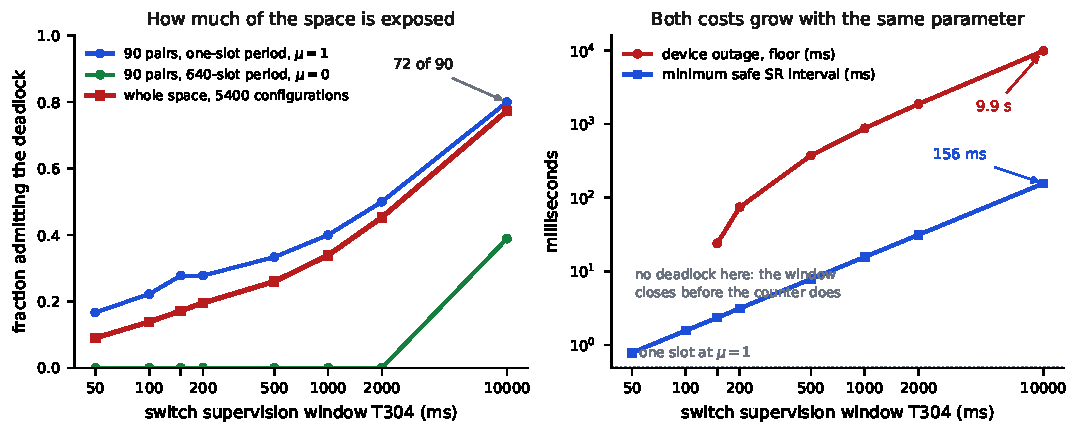
\includegraphics[width=\textwidth]{figures/atk16_space.pdf}
  \caption{Left: Percentage of configurations reaching deadlock versus \texttt{t304} duration. Right:
  Deadlock outage duration $T_{\text{dead}}$ trade-off.}
  \label{fig:space}
\end{figure}

As shown in \cref{fig:space}, deadlock is reached in 9.0\% of configurations at $\texttt{t304}=50$\,ms,
increasing to 27.8\% at 200\,ms, and reaching 77.4\% at 10\,s. In terrestrial deployments where
$\texttt{t304}=200$\,ms is standard, counter exhaustion induces an average dead interval of
$T_{\text{dead}} \approx 72$\,ms. With longer switch windows, $T_{\text{dead}}$ exceeds several seconds.

\section{The Safe Configuration Rule}
\label{sec:rule}

From \cref{eq:exhaust}, counter exhaustion occurs before T304 expiry whenever $T_{\text{exhaust}} < \texttt{t304}$.
Consequently, an operator can guarantee immunity from this deadlock if and only if:
\begin{equation}
  \texttt{sr-TransMax} \times T_{\text{interval}} \;\ge\; \texttt{t304}.
  \label{eq:rule}
\end{equation}
When \cref{eq:rule} is satisfied, T304 expires prior to counter exhaustion, safely invoking the standard
RRC connection re-establishment procedure.

\begin{table}[htbp]
  \centering
  \caption[Minimum safe SR interval satisfying Equation~(5.2)]{Minimum SR interval required to satisfy \cref{eq:rule} at $\texttt{sr-TransMax}=64$, and resulting latency penalty relative to 0.5\,ms baseline. The final row applies to Non-Terrestrial Network (NTN) supervision windows; terrestrial deployments use $\texttt{t304} \le 1$\,s.}
  \label{tab:rule}
  \small
  \begin{tabularx}{\textwidth}{@{}X c c r@{}}
    \toprule
    \texttt{t304} Duration & Minimum Safe SR Interval & Minimum \texttt{sr-ProhibitTimer} & Latency Penalty \\
    \midrule
    100\,ms   & 1.56\,ms   & \texttt{ms2}   & $3.1\times$ \\
    200\,ms   & 3.13\,ms   & \texttt{ms4}   & $6.2\times$ \\
    1000\,ms  & 15.63\,ms  & \texttt{ms16}  & $31.2\times$ \\
    10\,s (NTN) & 156.25\,ms & \texttt{ms192} & $312.5\times$ \\
    \bottomrule
  \end{tabularx}
\end{table}

However, enforcing \cref{eq:rule} imposes a severe performance trade-off (\cref{tab:rule}): at
$\texttt{t304}=200$\,ms, ensuring safety requires stretching the SR interval by $6.2\times$, degrading
application latency. Furthermore, 3GPP Release~19 dynamically selects the SR configuration via a 3-bit index in the
unauthenticated LTM Cell Switch Command MAC CE, bypassing static deployment audits.

\section{Independent Deployment Verification (Amarisoft)}
\label{sec:deployed}

We verified the parameters of both findings against a published commercial LTM setup from
Amarisoft~\cite{amarisoft2026ltm} (\cref{tab:deployed}).

\begin{table}[htbp]
  \centering
  \caption{Audit of published Amarisoft commercial LTM configuration~\cite{amarisoft2026ltm}.}
  \label{tab:deployed}
  \small
  \begin{tabularx}{\textwidth}{@{}p{5.0cm} p{3.2cm} X@{}}
    \toprule
    Configuration Parameter & Commercial Value & Security Verdict \& Finding \\
    \midrule
    \texttt{zero\-Correlation\-Zone\-Config} & 15 (Window: 46.4 units) & \textbf{Vulnerable to Finding~1} ($P(\text{capture})=0.78$) \\
    \texttt{sr-TransMax} & \texttt{n64} & Safe under default $\texttt{t304} = 1000$\,ms ($T_{\text{exhaust}} = 1280$\,ms) \\
    SR Periodicity / Prohibit & \texttt{sl40} (20\,ms) / absent & Governs escalation time ($T_{\text{exhaust}} = 1.28$\,s) \\
    \texttt{t304} Supervision Window & \texttt{ms1000} (1000\,ms) & \textbf{Vulnerable to Finding~2} if operator configures $\texttt{t304} \ge 2000$\,ms \\
    \bottomrule
  \end{tabularx}
\end{table}

The deployment chooses ZCZ~15, exposing a wide 46.4-unit search window that leaves Finding~1 completely
effective. For Finding~2, the vendor configured a conservative 20\,ms SR periodicity, rendering it
safe at $\texttt{t304}=1000$\,ms, but exposing it whenever $\texttt{t304}$ is set to 2\,s or higher.

\section{Inadequacy of Existing Defenses}
\label{sec:detect}

We evaluated four existing cellular defense mechanisms:
\begin{itemize}\itemsep2pt
  \item \textbf{Standardized 3GPP Counters (TS~28.552~\cite{3gpp28552}):} 3GPP performance management
        defines counters for handover execution, but contains no counter tracking intra-handover
        interruption duration. Deadlocked UEs simply appear as silent drops after T304 expiry.
  \item \textbf{Successful Handover Report (SHR, TS~38.300~\cite{3gpp38300}):} SHR records slow switches
        based on elapsed fractions of T304. However, it cannot distinguish between RF channel fading and
        corrupted \TA{}.
  \item \textbf{Dey and Patra's Handover Classifier~\cite{dey2025secure}:} This detector localizes
        adversaries using features observed during failure. In our attack, the relay acts during early
        acquisition and departs; by the time the switch executes, the attacker is absent, rendering
        real-time localization ineffective.
  \item \textbf{MAC CE Integrity Protection (TR~33.801-01~\cite{3gpp33801}):} Cryptographic signing of
        MAC CEs does not prevent the attack. The candidate \TA{} measurement itself is corrupted prior to
        encapsulation; thus, the gNB will compute a valid integrity tag over the already-corrupted \TA{}.
\end{itemize}

\chapter{Conclusion, Limitations and Future Work}
\label{ch:conclusion}

\section{Summary of Contributions}

This report investigated the architectural security of Lower-Layer Triggered Mobility (LTM) in
5G-Advanced and emerging 6G systems. Rather than focusing on unauthenticated MAC Control Element payloads,
this research evaluated the vulnerabilities created by LTM's core performance optimizations: pre-cached
candidate state, unauthenticated asynchronous timing advance acquisition, and RACH-less switching. Two
fundamental findings were identified through systematic 3GPP specification analysis and validated via
open-source simulation:

\begin{enumerate}\itemsep3pt
  \item \textbf{Finding 1 --- Corrupted Early Timing Advance (\cref{ch:m1}):} Early \TA{} acquisition
        records physical-layer preamble measurements that are bound only to an occasion and preamble
        index, without binding to a UE identity. Furthermore, 3GPP standards impose no retention limits
        on this network-cached value. An adversary using a low-power RF relay can forward preambles with
        excess delay. Measured on srsRAN and OAI, the decodability boundary spans 6--8 units (median 7):
        deterministic uplink failure under flat-fading/AWGN channel conditions by 8 units, with realistic
        multipath saturating slightly more gradually across the same range. As derived in
        \cref{eq:cp9}, this failure boundary is invariant across all 5G and 6G numerologies. The relay
        requires only a $+9.9$\,dB power advantage under flat fading
        ($+5.3$\,dB under multipath), operating from any location closer to the candidate cell than the
        victim.
  \item \textbf{Finding 2 --- Scheduling Request Deadlock (\cref{ch:m2}):} In TS~38.321 clause~5.4.4,
        exhaustion of the Scheduling Request counter (\texttt{SR\_COUNTER}) triggers unconditional
        deallocation of PUCCH, SRS, and all uplink/downlink grants at nesting depth \texttt{5>}. The recovery
        action (initiating Random Access) sits at depth \texttt{6>}, gated by a condition that evaluates
        to false during a RACH-less LTM switch. Formal evaluation across all 5400 legal 3GPP configurations
        shows that this deadlock is reachable in up to 77.4\% of configurations, silencing the UE until
        supervision timer T304 expires.
  \item \textbf{Deterministic Vulnerability Trigger:} Finding~1's corrupted \TA{} is what feeds Finding~2's
        deadlock: the same misalignment that fails the uplink transport block also decorrelates the PUCCH
        Format~0 Scheduling Request (\cref{ch:m2}), driving counter exhaustion with near certainty under
        flat fading and with high probability under multipath. The one escape clause~5.4.4 leaves
        open---a network-issued dynamic grant---does not save the UE, because the same corrupted \TA{}
        that caused the failure makes that grant undecodable too (\cref{sec:m2dyngrant}).
  \item \textbf{Safe Configuration Rule:} We derived the closed-form configuration rule
        $\texttt{sr-TransMax} \times T_{\text{interval}} \ge \texttt{t304}$ that ensures T304 expires
        prior to counter exhaustion, avoiding deadlock at the expense of increased scheduling latency.
\end{enumerate}

\section{Limitations of the Study}
\label{sec:limits}

The theoretical and specification-level findings in this report rest on normative 3GPP specifications
checked clause-by-clause. Several experimental limitations apply to the current phase of work:
\begin{enumerate}\itemsep2pt
  \item \textbf{Simulation-Based Evaluation:} Results are established using open-source protocol stacks
        (srsRAN, OpenAirInterface) and channel emulation models (3GPP TR~38.901). Live over-the-air
        testing on commercial hardware or custom RF relay prototypes was not performed in this phase.
  \item \textbf{Decoupled Stage Modeling:} Physical-layer preamble capture, transport block decodability,
        and Scheduling Request deadlock were evaluated using independent, targeted simulations across
        open-source stacks (srsRAN and OAI). A fully integrated, live multi-node cellular testbed running
        the relay, candidate gNB-DU, and UE MAC stack end-to-end remains an objective for Phase~II.
  \item \textbf{Channel and Receiver Assumptions:} Uplink baseline evaluations utilized single-antenna
        data reception and slot-static channel conditions, although receive diversity was fully swept for
        the control channel.
  \item \textbf{Receiver-Implementation Sensitivity:} The 6--8 unit decodability boundary is measured
        against srsRAN's and OpenAirInterface's specific receiver implementations (channel estimation,
        equalization, and tracking-loop design). Prior work on serving-cell TA manipulation against
        commercial UEs reports a substantially larger RLF-triggering error of 20--60 units
        (\cref{sec:lit-ta}), though that work measures a different failure mode (sustained downlink
        out-of-sync counting) against a different target (the active serving-cell link, under closed-loop
        tracking) than the one-shot coded-BLER cliff measured here against a freshly-acquired candidate
        \TA{}. Whether a production gNB's receiver chain would shift this report's specific 6--8 unit
        boundary is not established in this phase and is left open for further study.
  \item \textbf{Deployment Verification Scope:} Commercial verification was performed against published
        configuration dumps from one vendor (Amarisoft Callbox); wider multi-operator configuration surveys
        remain open.
\end{enumerate}

\section{Future Work}
\label{sec:future}

Phase II will focus on researching and evaluating, through further specification analysis and simulation,
defense mechanisms against the vulnerabilities identified in this phase. The urgency of this work only
grows with 6G numerologies: by \cref{eq:cp9}, the 7-unit failure boundary scales with $T_{\mathrm{unit}}$
and is invariant across subcarrier spacings as an algebraic property of 3GPP's own definitions of
$T_{\mathrm{unit}}$ and $\Delta f$. In upper mid-band (7--24\,GHz) and sub-THz 6G bands, $T_{\mathrm{unit}}$
shrinks from 260\,ns down to 65\,ns ($\mu=3$), compressing the absolute physical time budget available to
absorb a corrupted \TA{} from $1.82\,\mu\text{s}$ to $0.46\,\mu\text{s}$---so any remediation studied now
should be re-examined against that narrower margin for 6G.

\begin{enumerate}\itemsep3pt
  \item \textbf{Protocol \& Specification Hardening:} Refine the TS~38.321 clause~5.4.4 remediation already
        derived in this phase from the clause~5.2 CLTM precedent (\cref{sec:m2gap})---re-aligning resource
        deallocation with recovery actions so that a UE undergoing RACH-less switching retains a fallback to
        Random Access upon counter exhaustion---and examine analogous hardening of the early \TA{} acquisition
        and retention path (\cref{sec:m1retention}) at the specification level.
  \item \textbf{Defensive Telemetry \& Verification:} Study, through specification analysis and simulation,
        network-side defenses that bound and cross-check early timing advance measurements before they are
        applied (including retention limits on cached candidate state and cross-layer consistency checks),
        and physical-layer detection approaches for the multi-path delay and power-delay anomalies
        characteristic of RF relay forwarding.
\end{enumerate}


% ---------------------------------------------------------------------
%  BIBLIOGRAPHY
% ---------------------------------------------------------------------
\clearpage
\addcontentsline{toc}{chapter}{References}
{\footnotesize
\bibliographystyle{IEEEtran}
\bibliography{references}
}

\end{document}
